\documentclass[../main-v1.tex]{subfiles}
\begin{document}
\chapter{Use Cases}
\label{ch:use}
\newcommand{\ignore}[1]{{}}



\section{Introduction}

To introduce the \dword{tr} level processing issues for \dword{dune} computing, we describe some of the known use cases.  We start with  the experience gained from  \dword{proto},  using lessons learned from the 2018 run to understand the performance of future near and far detector modules. 

In addition to the challenges faced by HL-LHC experiments, as described in the HSF White Paper \cite{HEPSoftwareFoundation:2017ggl} DUNE, along with some dark matter and astrophysics experiments, faces considerable challenges in extracting very weak signals from large volumes of noisy data.  This additional challenge places strains on memory management beyond those anticipated at collider experiments. 

\section{Data Acquisition and Storage}

Data Acquisition software and hardware are responsibilities of the \dword{daq} group, with significant interfaces to offline computing. Important factors include communication of calibration and configuration information between online and offline computing, high-speed networking for data, high-reliability networking for configuration and monitoring, and adequate disk and CPU on both ends of the connection to allow efficient data transfer and continued data collection in the event of an extended network interruption or subsystem failure on either end.

These considerations apply to \dword{proto}, where data taking occurs at CERN with offline databases and archival storage in the US,  and, in future, the far and near detectors in South Dakota. 

Current status and proposed solutions are discussed in Chapters \ref{ch:db}(Databases) and \ref{ch:netw}(Networking). 

\subsection{Data Transfer from the Experiment}
Data need to be buffered locally and then transferred to permanent storage at the host lab(s).  Transfer activities include the generation of descriptive metadata, file transfer, writing the files to permanent storage and integrity checks.  Once data are confirmed to have successfully reached permanent storage, the local buffer may be cleared.  Current specifications call for the local buffers at remote sites to be able to store 3-7 days worth of data or one supernova trigger record's worth ($\sim 500$ TB) at a minimum. 

%{\it Major concerns:  Network bandwidth and reliability between Sanford and Fermilab. The ability of host lab systems to absorb and redistribute those data quickly. }
{\it Major challenges: Here the major area of concern is the remote location of the far detectors and space and power limitations at both the detector level and the surface. Other challenges include  the need for adequate lossless data compression to prevent data volume explosion. Chapter \ref{ch:netw} describes the status and plans for networking.}

\subsection{Control, Configuration, Conditions and Calibrations}
%\subsubsection{Configuration and Monitoring}
In addition to large-scale data transfers, online data-taking configurations and conditions need to stored and communicated to the offline systems. High-reliability network connections are needed to ensure that control signals as well as configuration and monitoring information are exchanged between the remote sites, local control facilities and the host laboratory.
This is the responsibility of the Fermilab networking groups and the \dword{daq} consortia with input and assistance from offline computing. 


\subsubsection{Slow controls}
Data from slow-control and monitoring systems needs to be recorded for offline use.  Examples include set points and readback for high-voltage systems, pressure, temperature and the outputs of purity monitors. 

{\it Potential challenge: Commercial SCADA systems tie us to proprietary software which may have limited interfaces, require expensive licenses and need migration to new systems if the vendor stops support.  A legacy SCADA system may only operate with aging hardware.}

\subsubsection{Online calibrations}
Online calibration information, such as channel noise and gain information, needs to passed to the offline systems. 

%{\it No novel concerns.}

\subsubsection{Beam monitors}
Beam monitoring, either per spill for neutrino interactions, or per particle in the CERN test beams, needs to be recorded and made available for offline processing. 
The IFBEAM system used for NuMI is already in use for \dword{proto}.

\subsection{Monitoring information}
Local online monitoring of data and experimental conditions will be done by the \dword{daq} groups but fast feedback on data movement and quality will also need to be provided based on fast processing of a subset of the data transferred offsite. 

{\it No novel concerns but substantial effort will be needed to build and maintain the system over the lifetime of the experiment.}

\subsection{Offsite high-level data filtering}
This is not yet part of the data plan, but there may be a need for offsite filtering of data before it is written to permanent storage. 

{\it  Initiation of a High-Level Trigger offsite remains a possibility if the need arises. Local space, power and cooling issues make this difficult to do at Sanford.}

\subsection{Outputs from DAQ and monitoring}
At the end of data transfer and after acquisition of configuration information,  we assume that data, metadata and configuration/calibration/beam information from the detectors have been transferred to offline computing facilities and can them be distributed and reconstructed. 




\section{Simulation chain}

There is more description of the algorithms used in the relevant algorithms chapter \ref{ch:appl}.  

\subsection{MARS}
The \dword{mars}\cite{abs1} simulation is used in the design of the beamline and near detector systems and  for safety/environmental calculations.  It is a significant user of CPU time. 

{\it Unique challenge: the MARS codes are not available outside of Fermilab.}

\subsection{Beam simulations}
The \dword{lbnf} beamline is simulated using the \dword{g4lbnf} framework.  Inputs include random number seeds and the beamline and target region geometry and materials.  Outputs are flux files containing simulated neutrino trajectories.  The flux files contain sufficient information to allow reweighting based on interaction cross sections.  These flux files must be cataloged and made available to offline simulation jobs.

{\it Minor challenge:  Distribution of flux files to remote sites requires use of \dword{stashcache} and careful record keeping.}



\subsection{Neutrino event generation}
Neutrino event generators are used to simulate neutrino interactions within a detector volume.  Input requirements are the neutrino beam flux, random number seeds and the detailed detector geometry. The output is 4-vectors for final state particles, including short-lifetime decay chains.  DUNE currently uses \dword{genie}\cite{GENIE} as the default but other default generators are possible. 

{\it We can rely on strong international efforts to produce standard generators. One challenge is the complexity of integrating multiple simulation code versions into our framework to ensure that there is timely evolution of the generators used as the physics understanding evolves.}

\subsection{Non-beam interaction simulations}
Simulations of non-standard model physics (e.g. neutron decay) and of cosmic ray and rock muon backgrounds are also used. 

{\it No major concerns.}

\subsection{Detector Interaction simulation}
A detector simulation such as GEANT4\cite{Allison:2016lfl} or FLUKA\cite{Bohlen:2014buj} is used to simulate the interaction of the particles described by the 4-vectors produced by the event generator. Input requirements are the geometry and outputs are the tree of interactions and energy deposits in the detector materials. 
Energy thresholds need to be quite low, as the detector systems are sensitive to MeV-scale processes. The large uniform detector volumes in LAr detector compensate for the low thresholds by requiring fewer volume crossings in a typical particle trajectory.  

Hadronic cross section on liquid argon are not yet fully understood.  DUNE has developed a reweighting framework 
\dword{Geant4Reweight}\cite{Calcutt:2021zck} to allow reuse of existing simulation as interaction rates are refined.

{\it Major concern: Due to the high granularity and low energy thresholds, interaction records can become very large. Simulated protoDUNE records are currently 200-300 MB, substantially larger than the raw waveforms.}

\subsection{Detector Simulation}
LAr TPC's require detailed models of electron trajectories through a potentially charged fluid.  Photon detection requires ray tracing over long distances.  Once electrons and photons have been propagated to the detection systems, simulation of the electrical response must also be done. Inputs are the output of the detector simulation, charge distribution in the liquid, absorption parameters and the detailed readout system geometry. Outputs are simulated streams of bits in the electronics. 

{\it Challenges:  ProtoDUNE experience indicates that, although simulation is reasonably fast relative to reconstruction (3 to 1), memory utilization even for protoDUNE is very high in simulation jobs.  5-6 GB process sizes in memory are typical for 6 \dwords{apa}.  High energy \dword{fd} interactions are expected to span more detector volume and thus require even more memory. Multiple passes may be needed as pptimization of the electron trajectory model is recursive and generally requires multiple reconstruction passes. }

\subsection{Overlays}
An efficient method for accurately simulating backgrounds in high rate environments is to overlay the simulated interaction information on real data.  For example, the environment in \dword{proto} or the near detector includes multiple beam and rock muon interactions in the same readout as an interaction of interest.  Libraries of properly formatted raw data can be combined with simulated hits from a simulated event to yield a realistic simulation of an interaction in the real detector. This required a library of such interactions and careful matching of the running conditions of the external raw events to the desired simulated events. 

{\it Challenges: We have not yet integrated overlays into the experiment framework. To do this we will need to distribute large volumes of overlay data to remote sites while maintaining randomness. Other experiments such as MicroBooNE and MINERvA have done this successfully. }

\subsection{Reweighting}
If intermediate simulation steps  are stored they can be used to reweight interaction to reflect new knowledge about the underlying cross sections, neutrino flux, detector materials or detector properties. Examples include the \dword{ppfx} beamline simulation reweighting system and the implementation of different cross section and final state interaction models in event generators. 

{\it No major challenge, several reweighting packages have been developed for NuMI/DUNE \cite{Aliaga:2015wva, Calcutt:2021zck}.}

\subsection{End point}
At this point we should have simulated data that is equivalent to the raw data coming from the detector. The next step is calibration and reconstruction. In all cases descriptive metadata needs to be produced that would allow reproduction of the simulation. 

{\it Possible challenge:  How many and which intermediate steps need to be stored permanently in order to optimize storage vs CPU utilization.}



\section{Reconstruction}

%%%%%%%%%%%%%%%%%%%%%%%%%%%%%%%%


%\section{ProtoDUNEdata: raw data acquisition, cataloging and storage \hideme{Schellman - draft}}\label{sec:use:pdii-daq}



% \subsection{DAQ to Raw Data store \hideme{Schellman-draft}}
% The \dword{daq} and \dword{cisc} systems are expected to provide in close to real time:

% \begin{itemize}
%     \item Raw data from the \dword{tpc} and \dword{pd} detectors. 
%     \item Information on run and trigger configuration
%     \item Beam information
%     \item Information on detector conditions. For example, granular information on the \dword{hv} is needed to study and compensate for \dword{hv} fluctuations. 
%     \item Low level calibration constants such as gains that do not need extensive offline processing
    
% \end{itemize}


% The raw data are written to disk locally and then copied to the archive site (FNAL). Once the data are confirmed to be on tape, the local copy may be deleted.

% A second copy of the raw data will be stored in a different archive. 

% \subsection{Inputs to reconstruction}

% The run and trigger information, beamline  data, conditions and calibration constants are made available through separate data paths and stored in appropriate databases. In ProtoDUNE Run I, some of this information was transferred manually and stored in the \dword{sam} catalog.  DUNE document 22983 \cite{bib:docdb22983} describes the metadata strategy for ProtoDUNE II and DUNE. 

%Figure \ref{fig:ch:use:pdii} illustrates a typical reconstruction flow for ProtoDUNE data
\begin{dunefigure}
[Data flow diagram for standard ProtoDUNE reconstruction]
{fig:ch:use:pdii}
{Data flow diagram for standard ProtoDUNE data reconstruction. The central boxes show the processing steps while the right side shows the large scale data flow  and the left side shows the auxiliary information needed for processing. Thicker lines indicate particularly large data volumes.}
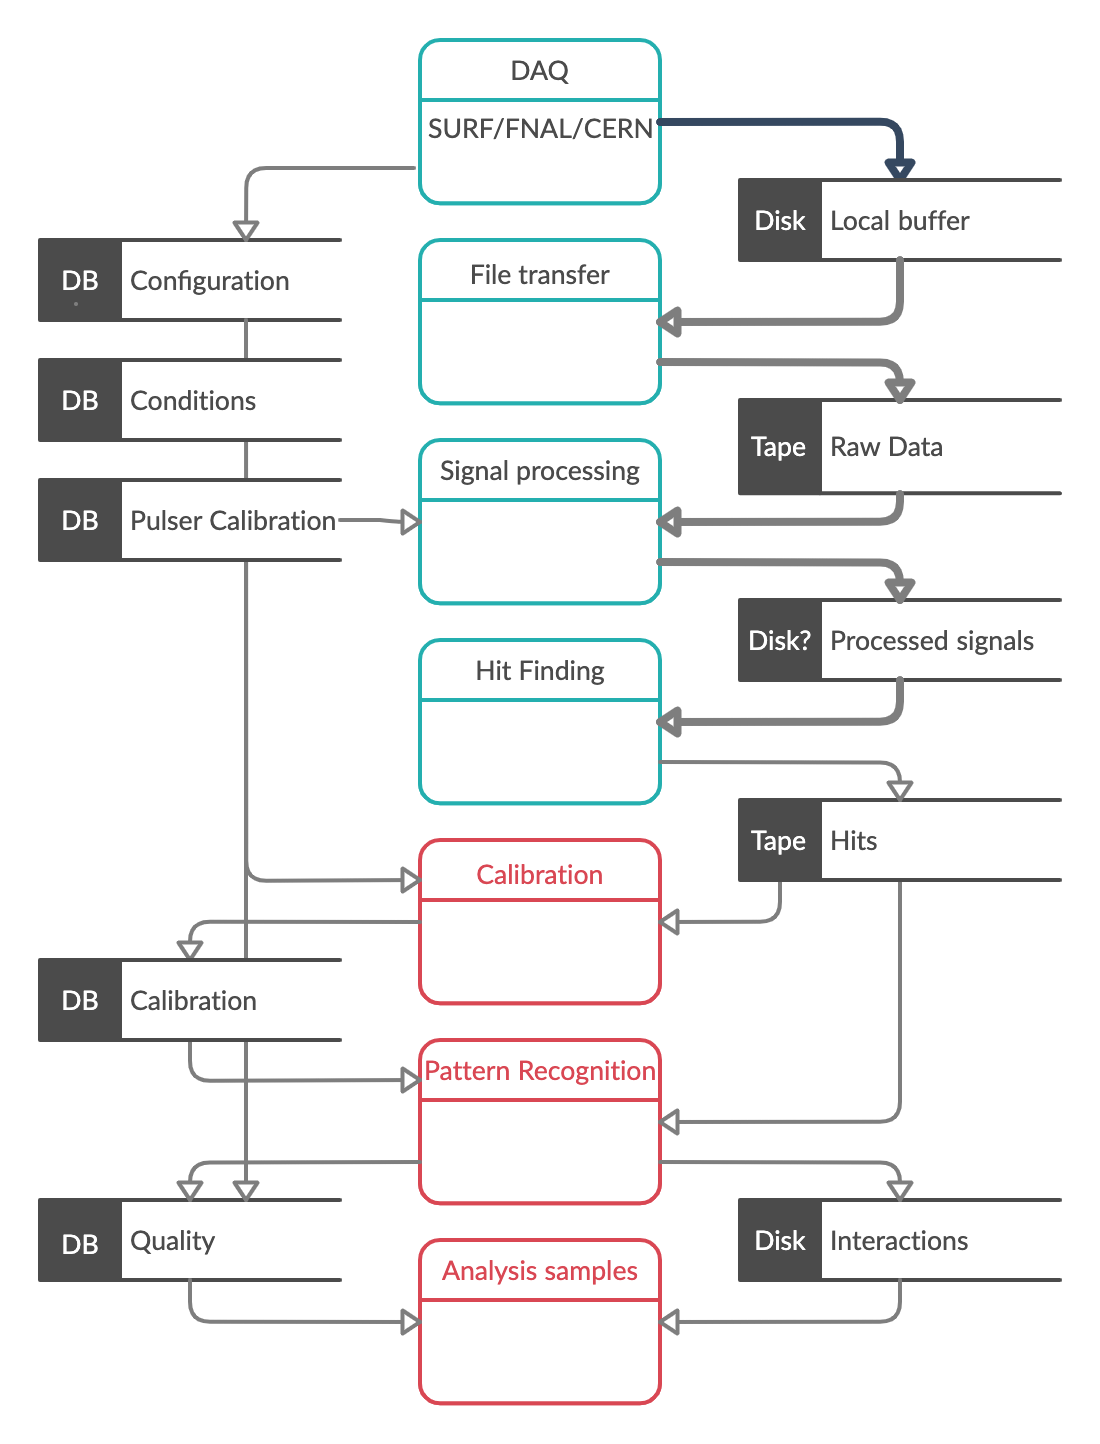
\includegraphics[width=0.8\textwidth]{graphics/IntroFigures/Data_processing_FD_v3.png}
\end{dunefigure}

\subsection{ProtoDUNE and Far Detector reconstruction\hideme{Schellman-draft}}\label{sec:use:pdii}

Figure \ref{fig:ch:use:pdii} shows the data flow for regular reconstruction in \dword{proto}.  There are in principle, multiple stages in reconstruction that are well suited to different computer architectures.  We expect the full \dword{fd} data processing to follow a similar path to that used by ProtoDUNE.  

Figure \ref{fig:ch:use:fdagg} illustrates  readout structures for full DUNE \dword{fd} modules.  A readout consists of a large number (up to 150) of   30 MB \dword{apa} readouts and a number of smaller readout fragments.  These need to be processed and then recombined into a single readout record. 

\begin{dunefigure}
[Data aggregation diagram for FD]
{fig:ch:use:fdagg}
{Data aggregation cases for the far detector. The top case shows information for normal beam or calibration readouts. A single file of $\sim 10$GB size contains several complete \dword{tr} with their boundaries designated by the dashed lines.  TPC \dword{apa}'s, Photon Detector (PD),  trigger primitives and a trigger  are recorded for each trigger readout.  In addition, a manifest which describes the relations between the data is stored, either in the file or in external metadata.  The bottom case is a supernova readout, in which thousands of 5-10 ms time slices must be read out over 100 sec.  The solid lines denote file boundaries. How data are ordered, by geographical position or by time is not  yet specified.}
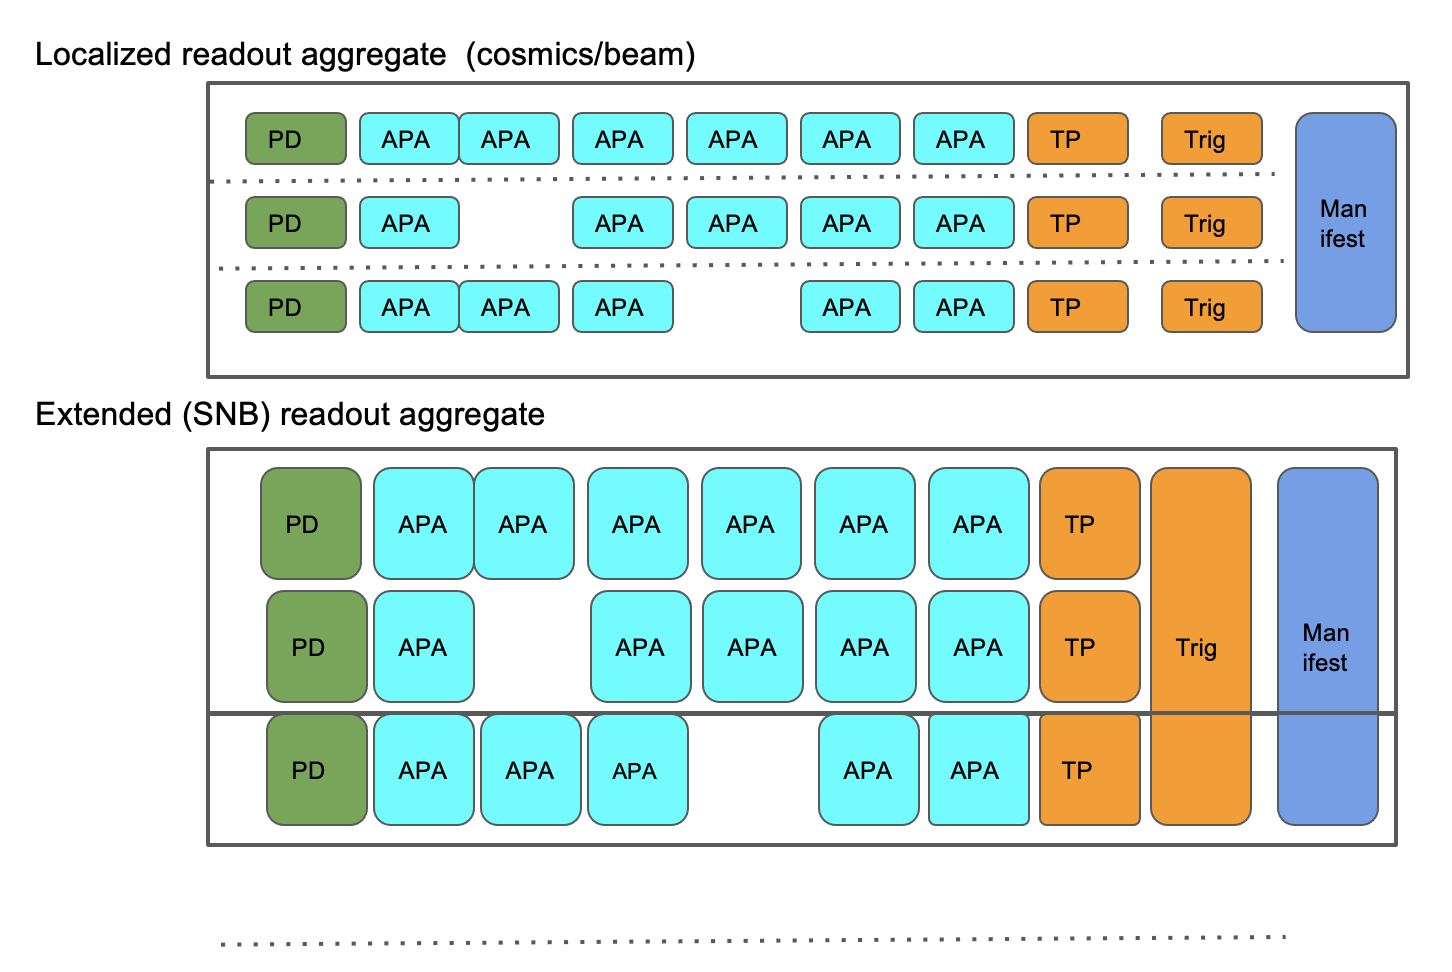
\includegraphics[width=0.8\textwidth]{graphics/IntroFigures/DataAggregation.png}
\end{dunefigure}
%\pagebreak

\subsubsection{Signal processing \hideme{Schellman-draft}}

This step takes the raw waveforms, applies  basic channel-to-channel calibrations, removes noise and stuck bits and performs 1 or 2D deconvolution.   In the \dword{tpc}, this processing step operates on large 2-D data arrays and may be suitable for different architectures than conventional pattern recognition. For the \dword{pd}, 1-D data arrays will be the input. It is anticipated that the signal processing step will not need to be done frequently. 

The input data at this point are quite uniform, effectively bit streams from \dword{tpc} and \dword{pd} channels.  There are correlations between channels in the \dword{tpc} data which require concurrent processing of multiple channels.  Segmentation at the level of a readout plane within an \dword{apa}  or \dword{lem} is desirable.  An uncompressed input \dword{apa} plane is of order 10 MB of 12-bit words. 

The output of this stage is still quite large even if lossless compression algorithms are applied. 

{\it Major challenge: The \dword{tpc} data need to be processed with a minimum granularity of a readout plane as multiple wires must be combined to achieve the best 2D deconvolution.  Each plane produces of order 10 million 12-bit samples/readout window. After decompression into 32 bit words, the input data size/APA is of order 30 MB per plane. This phase of data processing is well suited to parallel processing on GPU's or FPGA's but imposes new requirements on the event reconstruction framework. }

\subsection{Hit finding}
The processes signal information is then searched  for groups of  channels above threshold and fit to Gaussian pulses shapes.  This step is computationally quite different from the signal processing phase as it involves searching and fitting. 

The outputs are Gaussian fits to the pulses. This output is substantially smaller than the processed hit information. 

{\it The major challenge here is the radically different processing modality relative to hit finding.  Where hit finding can largely be implemented by matrix operations, hit finding algorithms make heavy use of code branching and external fitting algorithms. Accommodating both signal processing and hit finding on a single  architecture may be challenging. }

\subsection{Hits to Calibration \hideme{Schellman-draft}}

In this step, the processed hits from calibration samples (subsets of the full data, sometimes with special conditions) are run through specialized pattern recognition and used to derive high-quality calibration constants which are stored in the conditions database for future use.  Inputs include processed hit data but also detailed information about the configuration of the calibration system.  This step will likely be done many times, especially at experiment start. Calibration samples may be taken quickly and very large, for example 500 TB for a full laser calibration of the far detector. They will require occasional fast processing of PB scale data samples. 

{\it Major challenge: The large size of some calibration samples means that fast processing for monitoring and fast application will require peaks in data storage and processing at rates considerably higher than normal data taking.}

\subsection{Hits to reconstructed interactions }
In this step, the improved calibration constants and raw hits are input to the full  pattern recognition and reconstructed interactions are output. Data quality can be monitored as part of this processing and stored. 

Here a wide range of algorithms may be used. 

{\it Challenge:  At some point after either signal or  hit processing, the data from a full interaction must be brought together in memory in an appropriate format for pattern recognition. Each \dword{apa} can still produce up to 1 MB of hits, leading to memory footprints of up to 100 MB for pattern recognition inputs.}

\subsection{Data Streams}
At some point in the processing, specialized datasets and streams based on trigger type, reconstructed event information and intended use will be defined and produced.

\section{Production of Analysis samples}
The interaction data, which is in the output format supplied by the full reconstruction is reduced and reconfigured into analysis formats for use by users. 

In the long run this processing will be done as coherent production steps but may also be done by small groups while the data formats and procedures are being developed.

{\it Challenge:  This phase of processing is I/O limited and can put considerable strain on storage and network resources.  This and calibration drive the need to put most of the reconstructed data and simulation on disk at distributed sites as described in Part \ref{part:model}
A typical \dword{pdsp} data or simulation pass produces  10,000-100,000 2-8 GB reconstructed files and  then produces much smaller tuple outputs for analysis.  These reduction jobs stream using \dword{xrootd} and are IO bound. Preliminary monitoring studies indicate that average input rates of 5-30 MB/sec per process can be achieved within a single site, with aggregate rates of several GB/sec across multiple processes. We are currently mining data access records to measure rates and reliability as a function of source and sink. }

\subsection{Event classification}
Events will need to be classified.  Much of this is now done using ML techniques and is likely best done at the analysis phase rather than as part of the pattern recognition. 



\subsection{Data Analysis on reduced samples \hideme{Schellman/David/Calcutt - needs work}}
These are the samples users see and analyze when they are not developing new reconstruction  or calibration algorithms. 

Analysis samples should be useful and as small as possible.  Analysis codes should not need to read from the central databases but may access small local replicas. 

Data analysis may be done on local clusters, on collaboration grid facilities using shared data samples or in dedicated analysis facilities that offer advanced access methods (Caffea ...). 

An important question is what auxiliary information is needed and how it will be delivered. In particular, geometry and run quality information are often needed in final analysis stages while direct access to detailed electronics calibrations is less often needed. 

This phase of processing is typically very IO bound and requires fast access to smaller data samples. 

\subsection{Parameter estimation}
Once final data samples are available, parameter estimation needs to be done to extract model parameters.  The NOvA parameter estimation \cite{NOvA:2021nfi} involved exploring of order 100 sources of uncertainty and were performed on the \dword{nersc} HPC systems. 

\section{Additional Activities}

\subsection{Database design and access}
DUNE will need databases for a wide range of activities, from tracking detector construction to detailed calibration.  Chapter \ref{ch:db} describes the database planning in detail.  Major considerations are the ability to  receive inputs from a wide variety of sources, some of which may have proprietary interfaces and then to distribute information to a broad range of processing sites.   Use of open-source solutions is highly encouraged but may require additional effort.

{\it The major challenge for DUNE, as for most database projects in the field, is the sheer amount of effort needed to carefully specify multiple problems and then deploy solutions that work at scale. As the database schema will be largely unique to DUNE, we can take advantage of existing general tools but much of the design must be closely tailored to our needs. The problem itself is not novel but the solution will require a large fraction of the total software effort.}


\subsection{Machine Learning Training} 
Many reconstruction and simulation algorithms use \dword{ml} algorithms.  While these algorithms may run quickly, they   require significant resources to train.  

\subsection{Event Display}
Event displays are needed for all phases of simulation and reconstruction for algorithm validation, data monitoring and final result presentation. 

{\it The extremely large data content of LArTPC events makes the provision of fast/detailed and aesthetically pleasing displays challenging.  We have existing solutions but they tend to be slow and somewhat awkward to use.}

\subsection{Code Management and Releases}
DUNE  uses modern software frameworks (see \ref{ch:fworks} for a fuller description). The large number of detector components and algorithm developers requires careful attention to code and release management and to the build environment.  This is described in more detail in Chapter \ref{ch:codemgmt}

DUNE is migrating to github as the main code repository and SPACK for configuration.  

{\it One ongoing challenge will be managing the complex DUNE code stack across multiple architectures as operating systems and compilers evolve. Another challenge is making certain that downstream codes for calibration and analysis are consistently versioned and tracked for reproducibility.} 

\subsection{Continuous Integration and Code validation}

Part of code management and releases will be continuing validation of important algorithms as operating system, compilers and simulations evolve. 



\subsection{Documentation}
Tools for improved documentation are needed. DUNE currently relies on a wide range of tools, mostly open source.

\begin{description}
\item[Mediawiki] for general structured information
\item[docdb] \dword{docdb} is used for version-controlled documents. 
\item[edms] \dword{edms} is used for version-control project documentation.
\item[indico] \dword{indico} is used for presentations and meetings. 
\item[github] Github is increasingly used to document individual code packages.
\item[google tools] google docs and sheets are used for short term shared work on documents.
\item{Slack}  Many discussions now take place in Slack


\end{description}

{\it One major challenge is increased government  scrutiny of the release of potentially sensitive technical information.  An overly conservative strategy towards information sharing has a profound negative impact on the availability of web-based tools for creating, disseminating and searching for DUNE computing documentation. A parallel  challenge is that restrictive official tools lead to frequent use of ephemeral, unindexed tools such as google docs and Slack.  Documents created with those tools need to migrate (or be rewritten) to the permanent stores such as docdb or be lost.  } 

%We are currently missing a performant FAQ system and access to code browsers such as Doxygen. }

%Current tools include a wiki, github, docdb for version controlled documents, and indico for talks and tutorials.  Many development documents are created in online tools such as google docs and must be migrated by hand to docdb or other safer areas. 



\subsection{Training}
Training in offline software techniques is given twice yearly in association with  collaboration meetings.  A dedicated training team collaborates with the \dword{hsf} training group to create documentation based on the software carpentry framework and to record videos of tutorials for particular activities. This is describe in Chapter \ref{ch:train}

\subsection{User support}
User support is supplied by collaboration experts, the small DUNE core computing team and by the Fermilab and CERN IT groups. 
Users access help through the DUNE Slack channel or through ServiceNow requests to FNAL IT. 

% One outstanding issue is support for user batch job submission.  The \dword{project.py} xml based submission system developed by MicroBooNE is popular with users but only supported for that experiment.  

%\ignore{  % this section should appear elsewhere


%\fixme{need some text here on simulation}

\pagebreak


%Section on ProtoDUne simulation moved to the simulation chapter

%\section{Data reduction at FNAL before writing it out?}

%\section{Fast processing for data monitoring} 

\section{Normal  and SNB Far Detector: acquisition and reconstruction \hideme{Schellman - started} }
\label{sec:use:fdbeam}  %% fix label according to section

% \begin{dunefigure}
% [Data aggregation diagram for FD]
% {fig:ch:use:fdagg}
% {Data aggregation cases for the far detector. The top case shows information for normal beam or calibration readouts. A single file of $\sim 10$GB size contains several complete trigger readouts with their boundaries designated by the dashed lines.  TPC APA's, Photon Detector (PD),  trigger primitives and a trigger  are recorded for each trigger readout.  In addition, a manifest which describes the relations between the data is stored, either in the file or in metadata.  The bottom case is a supernova readout, in which thousands of 5-10 ms time slices must be read out over 100 sec.  The solid lines denote file boundaries. How data ordered, by geographical position or by team is not specified.}
% 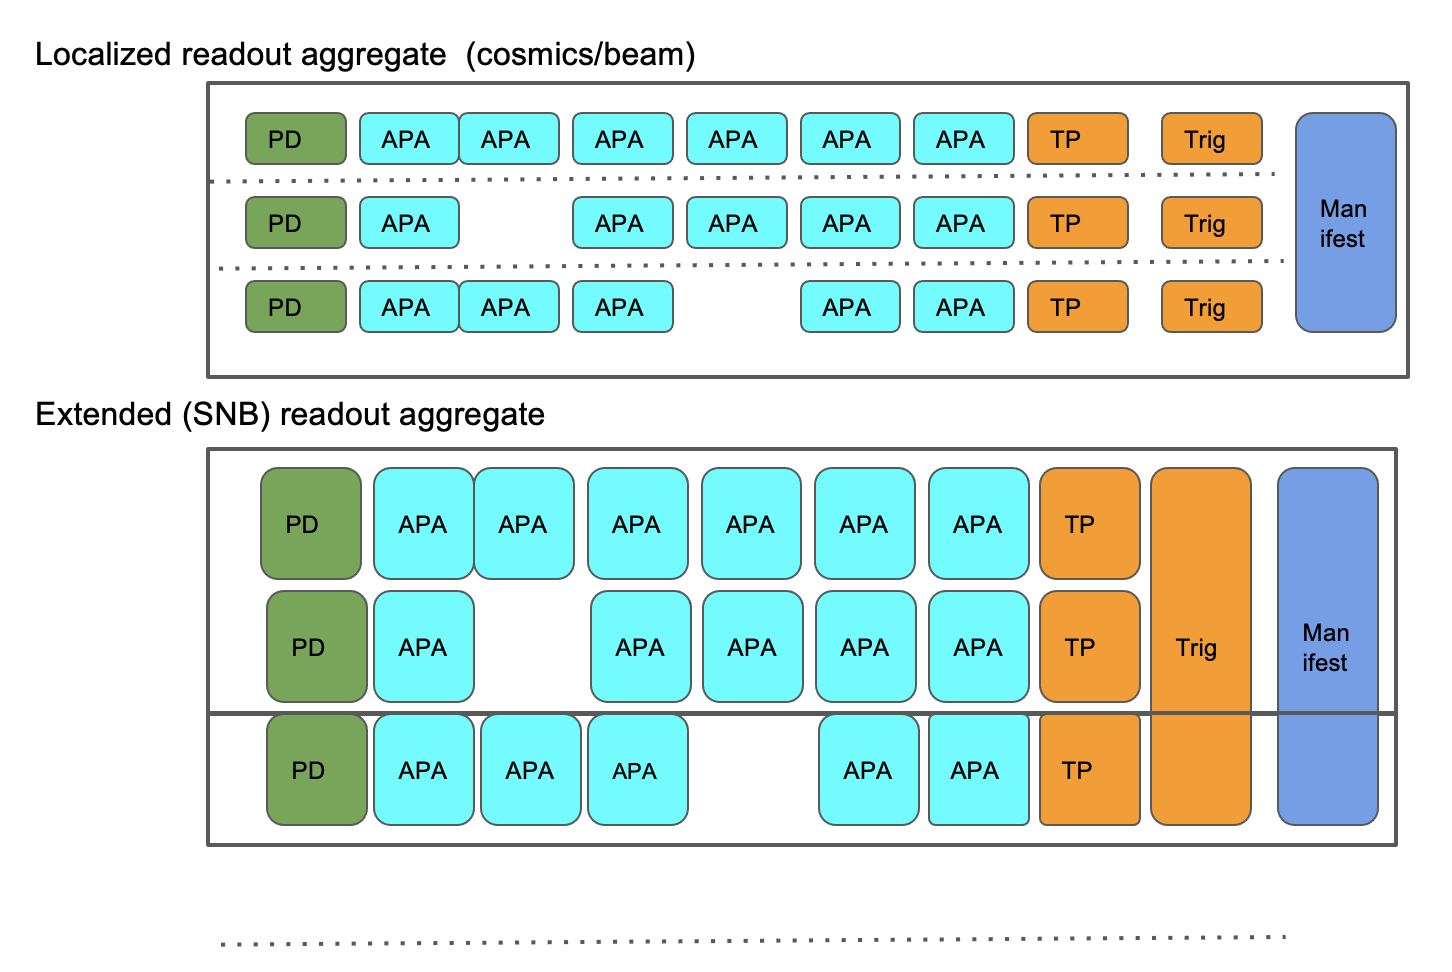
\includegraphics[width=0.8\textwidth]{graphics/IntroFigures/DataAggregation.png}
% \end{dunefigure}
% %\pagebreak

% \todo{Need more text on this case}

 
% \section{ND Beam Data: Beam data acquisition and reconstruction \hideme{ Mathew Muether/Tom Junk - needed}}
% \label{sec:use:ndbeam}  %% fix label according to section



% \section{DUNE Simulation \hideme{Junk/Schellman/Muether}}  \fixme{Mathews' diagram} 

% ND and FD data should be simulated using similar tools, differing in the detector layout but not the underlying generators. 

% \hideme\subsection{Need Mathew's diagram of the processing chain}

%\todo{how big are events?  what are memory/CPU requirements}

% \subsection{Beam simulation\hideme{Junk-draft}}\label{sec:use:beamsim}
% The neutrino beam is simulated using g4lbnf\cite{g4lbnf} a geant4\cite{geant4} based simulation of the beamline components.  Intermediate interactions are stored so that cross section reweighting can be applied.  The beam simulation is generally done separately and beam files are stored and used when needed. 

%\subsection{Cosmic simulation?}



% The far and near detectors subtend very different solid angles so one has to simulate a very large number of events or use reweighting techniques to properly cover both. 

% %\subsection{Cosmic simulation?}

% \subsection{Interaction simulation\hideme{Schellman-draft}}\label{sec:use:intmodel}
% Next an event generator is used to simulate the primary interaction.  This step requires a reasonably accurate geometry for the detectors to account for different target materials and, for the near detector, different locations. Simulation parameters and reasonably detailed event information need to be stored to allow for subsequent reweighting.  To date, most DUNE simulations have used the GENIE\cite{GENIE} event generator. 

% \subsection{Particle tracing\hideme{Junk-draft}}\label{sec:use:tracing}
% The geant4 simulation package is then used to simulate the energy deposited by final state particles as they pass through the detector.  Both ionization and scintillation signatures need to be recorded.  

% \subsection{Detector response simulation\hideme{Schellman-draft}}\label{sec:use:detsim}
% Once geant4 has simulated the energy deposit, detailed simulation of charge and light collection and electronics response can be done.  

% \subsection{Overlay\hideme{Schellman-draft}}\label{sec:use:overlay}
% It is often useful to overlay real data on simulated events to fully account for cosmic ray and upstream neutrino interactions. This adds complexity as the real data must be delivered to simulation jobs and be properly matched to the running conditions for the simulation.  The "electronics" signals from real data and simulation need to be mixed and stored.  The \dword{microboone} experiment has adapted \dword{larsoft} to do this and we plan to build on that experience. 

% \todo{Discussion of overlay experience from MicroBooNE \hideme{Kirby -needed}}

% \subsection{Reconstruction} \label{sec:use:mcreco}
% Reconstruction and analysis can then be performed using the same methods as in section \ref{sec:use:pdii}.  Due to the large amount of interaction and intermediate step information kept for studies, simulated events are often several times the size of real data.  A significant question, given the size of events, is whether it may be more efficient to regenerate than to store all the information needed for reweighting. 

% \subsection{Resource requirements for simulation and reconstruction \hideme{Schellman-Junk -needed}}
% \todo{add a table showing \# of events, CPU and memory footprint for each step}









% \section{Oscillation analysis} Chris Backhouse?  Chris Marshall? 
% \label{sec:use:osc}

% \section{Supernova data: acquisition and fast reconstruction}
% \label{sec:use:supernova}  %% fix label according to section

% \subsection{Fast ( 1 day turnaround)} \fixme{Priority for readout?}

% \subsection{Full Supernova}

% \section{Solar/BSM analysis}
% \label{sec:use:BSManalysis}

% \section{Calibration data: acquisition, reconstruction and use}
% \label{sec:use:calib}  %% fix label according to section

% \section{Hardware database use case} \fixme{Paul has an example}
% \label{sec:use:hdb} 

% \section{Analysis Facility}\todo{Claire}
% \label{sec:use:analysis}

% \section{What's missing?}
% \label{sec:use:todo}
% } % end of ignore
% \section{Data movement}
% An important component in computing is data placement.  DUNE will generate 30 PB/year and takes advantage of storage and CPU at multiple sites worldwide.  Our present model uses the Fermilab SAM system to track data locations.  Going forward, the Rucio\cite{Barisits:2019fyl} system will be used to move and locate large datasets (of order 100 TB) at DUNE storage sites.  The workflow and data dispatcher systems will then help users and processes find the most accessible copy of the data for their site. 

% \todo{Produce table that shows, input/output/CPU and memory footprint for each stage of processing - Heidi gathers info}



\end{document} % if using subfiles